\section{Real Data Application}
In this section, we conducted a real data application using data from fMRI painful stimulus study we introduced in section 2.  During this painful study, a total number of 20 subjects are asked for the subjective painful rating after corresponding thermal stimuli is given.  Following the thermal stimuli, fMRI machine records the brain activity every 2 seconds from 21 regions of interest (ROI) simultaneously at one's brain for a entire course of 46 seconds. Then the subjective painful rating regarding to the hot/warm stimuli is reported by the individual. For each individual, different amount of visits ranging in [39,48] are taken. We treat the continuously observed brain neural imaging data as a functional covariate, thermal stimuli as a binary categorical covariate,  and subjective rating as scalar response. Then  we applied our proposed functional mixed effect model extending the scalar on function linear
regression for this repeated outcomes.

Test procedures on 21 ROIs show that there are about half which have significant subjective-specific functional random effect at level of 0.05. We picked 3 out of the most significant ROIs (ROI 1, ROI 10, and ROI 19) to visualize difference among $\beta_i(t)$ and compare modeling them with no functional random effect and with heteroscedastic variance on subject-specific brain activity. Figure $\ref{betat}$ shows the

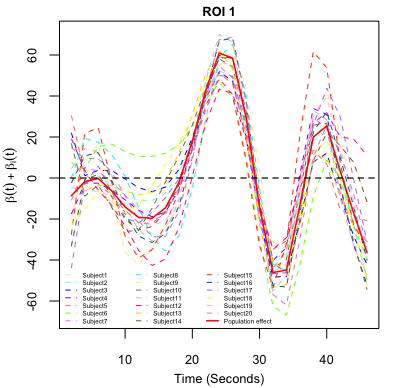
\includegraphics[width=0.48\textwidth]{ROI1_betat.png}
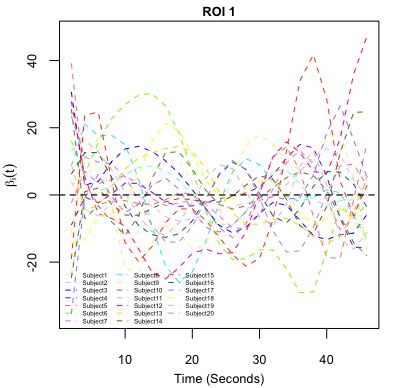
\includegraphics[width=0.48\textwidth]{ROI1_betait.png}

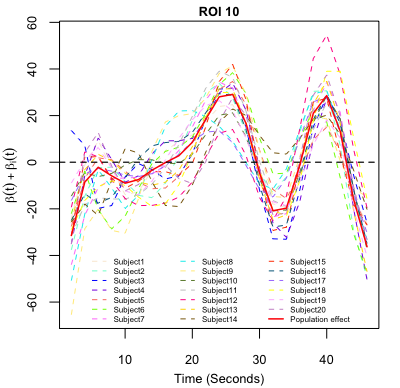
\includegraphics[width=0.48\textwidth]{ROI10_betat.png}
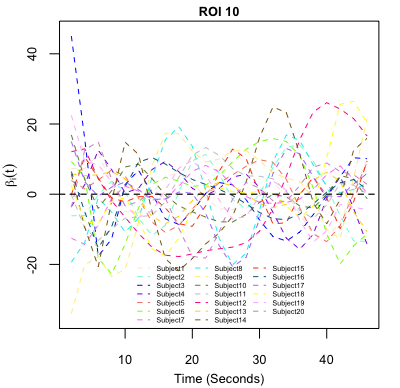
\includegraphics[width=0.48\textwidth]{ROI10_betait.png}

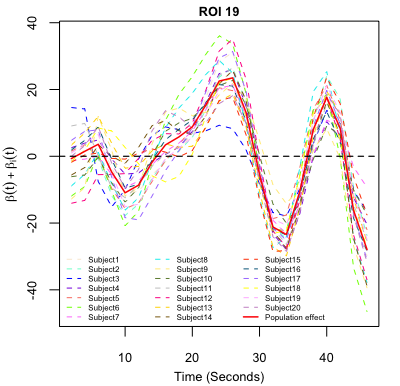
\includegraphics[width=0.48\textwidth]{ROI19_betat.png}
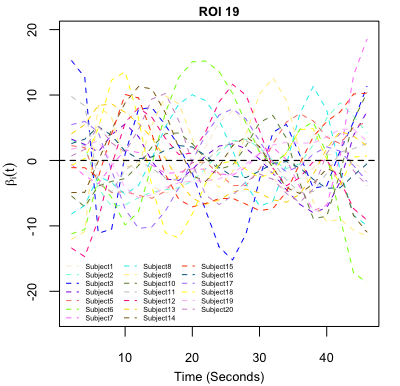
\includegraphics[width=0.48\textwidth]{ROI19_betait.png}

\begin{figure}[h!]
\centering
\caption{Estimates of subject-specific functional mediation effects and subject deviation from the population functional mediation for ROI 1, 10 and 19. In the left panel, the red solid line represents the population functional mediation effect  $\beta(t)$; each of the dashed curve is subject-specific functional mediation effect $ \beta(t) + \beta_i(t)$; In the right panel, each of  the dashed curve is subject-specific deviation $\beta_i(t)$ from the population functional mediation effect $ \beta(t)$. Each subject has the same color across all ROIs.}
\label{betat}
\end{figure}



\begin{table}[!h]
 \caption{RMSE comparison of three models for ROI 1, 10, and 19}   
 \centering
\begin{tabular}{ c | c   c   c  }\hline\hline
 \multirow{2}{*}{ROI}
  & \multicolumn{3}{c}{RMSE}  \\ \cline{2-4}
  & No random effect  & Homogeneous & Heteroscedastic \\
  \cline{1-4}
ROI 1 &  79.236  & 74.181 & 73.67 \\ \cline{1-4}
ROI 10 & 80.649 & 74.59 &  74.64 \\ \cline{1-4}
ROI 19 & 80.39 & 76.37 & 76.67\\
\hline
\hline
 \end{tabular}  
\end{table}
  
%  \begin{table}
%\begin{tabular}{| l | l | l | l | l |}\hline
  %\multirow{1}{*}{Model}  &  & MSE & RMSE & MSE* \\ \cline{1-5}
 %\multirow{2}{*}{Voxel 1}
  %& \multirow{1}{*}{No random effect} & 6278.428 & 79.236 & 6269.934  \\ \cline{2-5}
 % & \multirow{1}{*}{Heterskedastic} & 5428.054 & 73.67 & 5424.417  \\ \cline{2-5}
 % & \multirow{1}{*}{Our model} &  5502.77& 74.181& 5500.03 \\ \cline{2-5}  
 %  \multirow{2}{*}{Voxel 10}
%  & \multirow{1}{*}{No random effect} & 6504.301 & 80.649 & 6496.561  \\ \cline{2-5}
%  & \multirow{1}{*}{Heterskedastic} & 5572.025 & 74.64 & 5570.738  \\ \cline{2-5}
%  & \multirow{1}{*}{Our model} &  5564.165 & 74.59 & 5561.549 \\ \cline{2-5}
%     \multirow{2}{*}{Voxel 19}
%  & \multirow{1}{*}{No random effect} & 6463.045 & 80.39 & 6452.72  \\ \cline{2-5}
%  & \multirow{1}{*}{Heterskedastic} & 5879.517 & 76.67 & 5873.454  \\ \cline{2-5}
%  & \multirow{1}{*}{Our model} &  5833.417& 76.37 & 5826.98 \\ \cline{1-5}
% \end{tabular} 
%  \caption{Model fitting comparison}    
%\end{table}
  
 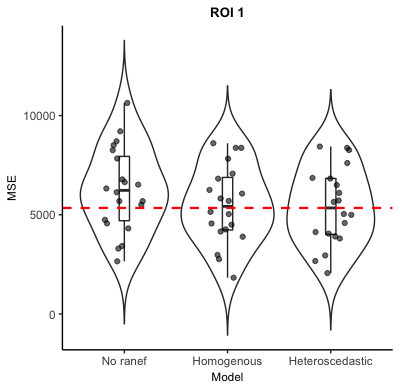
\includegraphics[width=0.45\textwidth]{ROI1_voilin.png}
 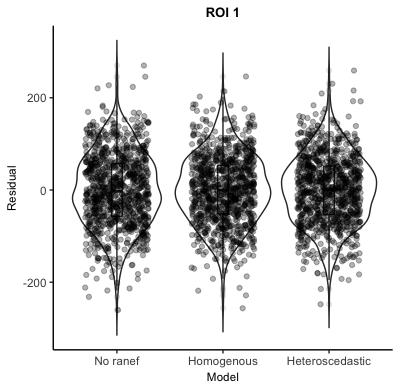
\includegraphics[width=0.45\textwidth]{ROI1_voilin_resi.png}
 
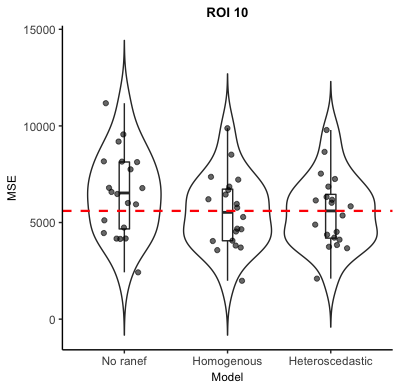
\includegraphics[width=0.45\textwidth]{ROI10_voilin.png}
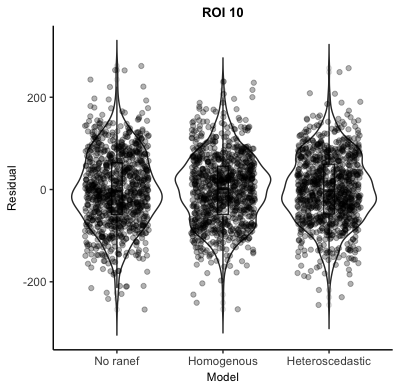
\includegraphics[width=0.45\textwidth]{ROI10_voilin_resi.png}

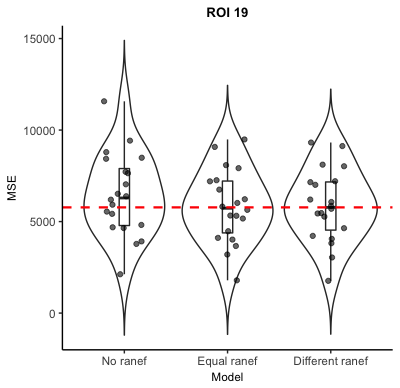
\includegraphics[width=0.45\textwidth]{ROI19_voilin.png}
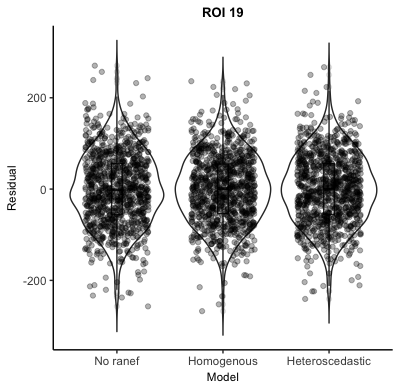
\includegraphics[width=0.45\textwidth]{ROI19_voilin_resi.png}

\begin{figure}[h!]
\centering
\caption{Comparison of model fitting among three models for ROI 1, 10 and 19.  Left panel shows the violin plot for MSE of each of 20 subjects in three models; right panel shows the violin plot for 943 residuals in three models. The red dashed curve represents the median MSE given by Model with heteroscedastic variance}
\label{MSE_voilin}
\end{figure}

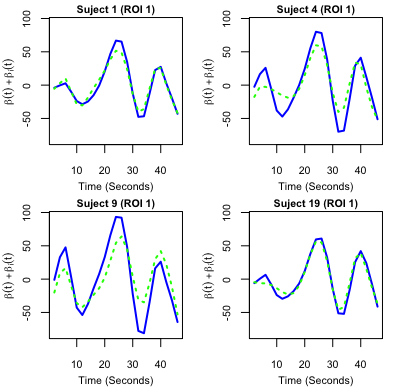
\includegraphics[width=0.45\textwidth]{ROI1_sub4_betat.png}
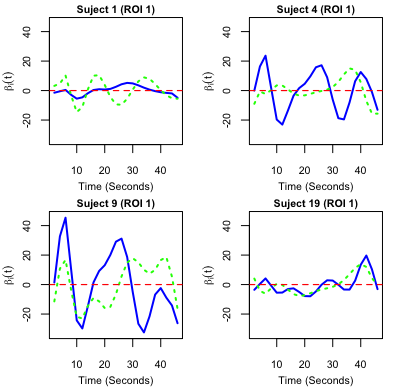
\includegraphics[width=0.45\textwidth]{ROI1_sub4_betait.png}

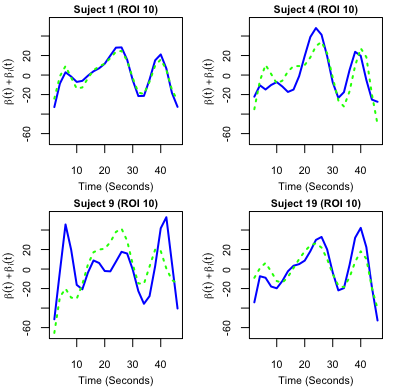
\includegraphics[width=0.45\textwidth]{ROI10_sub4_betat.png}
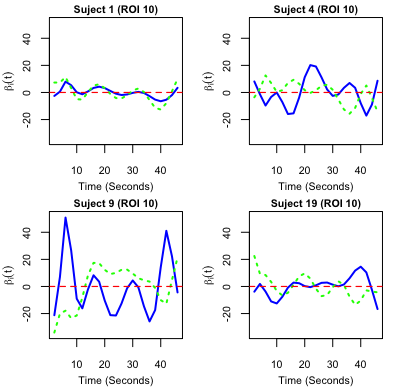
\includegraphics[width=0.45\textwidth]{ROI10_sub4_betait.png}

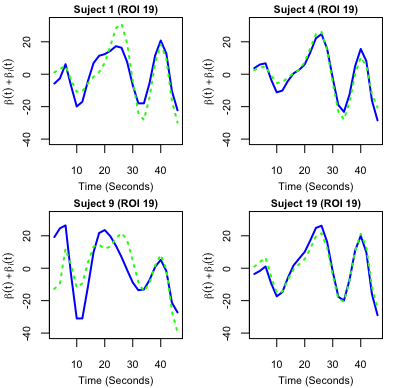
\includegraphics[width=0.45\textwidth]{ROI19_sub4_betat.png}
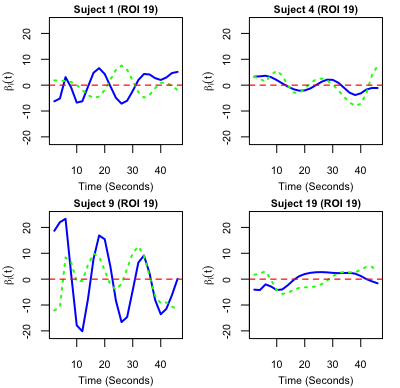
\includegraphics[width=0.45\textwidth]{ROI19_sub4_betait.png}

 \begin{figure}[h!]
\centering
\caption{Comparison of estimates of subject-specific functional mediation effects and subject deviation from the population functional mediation of subject1, subject4, subject9, and subject 19 for ROI 1, 10 and 19. In the left panel, the blue solid line represents subject-specific functional mediation effect $ \beta(t) + \beta_i(t)$ given by model with heteroscedastic variance, the green dash line represents $ \beta(t) + \beta_i(t)$ given by model with homogeneous variance; In the right panel, the blue solid line represents subject-specific functional mediation effect  deviation from the population effect $\beta_i(t)$ given by model with heteroscedastic variance, the green dash line represents $\beta_i(t)$ given by model with our method}
\label{voxel 4sub}
\end{figure}

